\documentclass[12pt]{report}
\usepackage[utf8]{inputenc}
\usepackage[russian]{babel}
%\usepackage[14pt]{extsizes}
\usepackage{listings}
\usepackage{graphicx}
\usepackage{amsmath,amsfonts,amssymb,amsthm,mathtools} 
\usepackage{pgfplots}
\usepackage{filecontents}
\usepackage{indentfirst}
\usepackage{eucal}
\usepackage{amsmath}
\usepackage{enumitem}
\frenchspacing

\usepackage{indentfirst} % Красная строка


%\usetikzlibrary{datavisualization}
%\usetikzlibrary{datavisualization.formats.functions}

\usepackage{amsmath}


% Для листинга кода:
\lstset{ %
language=caml,                 % выбор языка для подсветки (здесь это С)
basicstyle=\small\sffamily, % размер и начертание шрифта для подсветки кода
numbers=left,               % где поставить нумерацию строк (слева\справа)
numberstyle=\tiny,           % размер шрифта для номеров строк
stepnumber=1,                   % размер шага между двумя номерами строк
numbersep=5pt,                % как далеко отстоят номера строк от подсвечиваемого кода
showspaces=false,            % показывать или нет пробелы специальными отступами
showstringspaces=false,      % показывать или нет пробелы в строках
showtabs=false,             % показывать или нет табуляцию в строках
frame=single,              % рисовать рамку вокруг кода
tabsize=2,                 % размер табуляции по умолчанию равен 2 пробелам
captionpos=t,              % позиция заголовка вверху [t] или внизу [b] 
breaklines=true,           % автоматически переносить строки (да\нет)
breakatwhitespace=false, % переносить строки только если есть пробел
escapeinside={\#*}{*)}   % если нужно добавить комментарии в коде
}

\usepackage[left=2cm,right=2cm, top=2cm,bottom=2cm,bindingoffset=0cm]{geometry}
% Для измененных титулов глав:
\usepackage{titlesec, blindtext, color} % подключаем нужные пакеты
\definecolor{gray75}{gray}{0.75} % определяем цвет
\newcommand{\hsp}{\hspace{20pt}} % длина линии в 20pt
% titleformat определяет стиль
\titleformat{\chapter}[hang]{\Huge\bfseries}{\thechapter\hsp\textcolor{gray75}{|}\hsp}{0pt}{\Huge\bfseries}


% plot
\usepackage{pgfplots}
\usepackage{filecontents}
\usetikzlibrary{datavisualization}
\usetikzlibrary{datavisualization.formats.functions}

\begin{document}
%\def\chaptername{} % убирает "Глава"
\thispagestyle{empty}

Ограничения, которые, я наложил, чтобы достичь результата:

\begin{itemize}
	\item на вход сортировке подается отсортированный массив;
	\item pivot каждый раз берется последний элемент;
	\item размер элемента массива достаточно большой;
	\item размер массива достаточно большой.
\end{itemize}

В качестве элемента массива, я взял структуру, размер которой (на моей машине) составляет 32 байта (Листинг 1). Размер сортируемого массива - 100000
элементов.

\begin{lstlisting}[label=some-code,caption=Элемент сортируемого массива, language=C]
typedef struct {
	size_t a;
	size_t b;
	size_t c;
	size_t d;
} my_struct_t;
\end{lstlisting}

\begin{lstlisting}[label=bsort,caption=Функция сортировки массива пузырьком, language=C]
#define SWAP(t, a, b) do { t c = a; a = b; b = c; } while (0);

void bubble_sort(check_t arr[], int size) {
	for (int i = 0; i < size - 1; i++) {
		for (int j = 0; j < size - i - 1; j++) {
			if (arr[j].a > arr[j + 1].a) {
				SWAP(my_struct_t, arr[j], arr[j + 1]);
			}
		}
	}
}
\end{lstlisting}

\begin{lstlisting}[label=qsort,caption=Функция быстрой сортировки, language=C]
#define SWAP(t, a, b) do { t c = a; a = b; b = c; } while (0);

void my_qsort(my_struct_t arr[], int start, int stop) {
	if (start >= stop) {
		return;
	}

	int left = start;
	int right = stop;
	check_t cur_el;

	my_struct_t mid = arr[right];

	while (left <= right) {
		cur_el = arr[left];

		while (cur_el.a < mid.a) {
			left += 1;
			cur_el = arr[left];
		}

		cur_el = arr[right];
		while (cur_el.a > mid.a) {
			right -= 1;
			cur_el = arr[right];
		}
		
		if (left <= right) {
			SWAP(my_struct_t, arr[right], arr[left]);
			left += 1;
			right -= 1;
		}
	}

	my_qsort(arr, start,  right);
	my_qsort(arr, left, stop);
}
\end{lstlisting}


\begin{figure}[h]
	\centering
	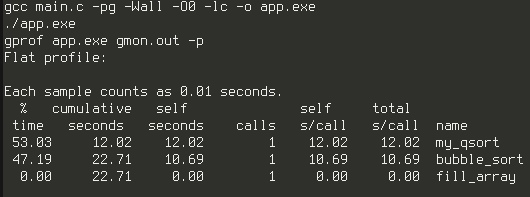
\includegraphics[scale=0.85]{re.jpg}
	\caption{Результаты замеров функций сортировки пузырьком и быстрой сортировки}
	\label{fig:mpr}
\end{figure}

Данный результат можно объяснить следующими факторами:

\begin{itemize} 
	\item на отсортированном массиве сортировка пузырьком только лишь сравнивает значения, но не переставляет никакие элементы в памяти;
	\item наооборот, при выбраном pivot быстрая сортировка делает много перемещений элементов массива в памяти;
	\item элементы массива весят достаточно много (32 байта), их swap в памяти занимает достаточно много времени;
	\item помимо перестановок в памяти, быстрая сортировка так же делает какие-либо сравнения элементов
\end{itemize}

\bibliographystyle{utf8gost705u}  % стилевой файл для оформления по ГОСТу

\bibliography{51-biblio}          % имя библиографической базы (bib-файла)


\end{document}
